%%%%%%%%%%%%%%%%%%%%%%%%%%%%%%%%%%%%%%%%%%%%%%%%%%%%%%%%%%%%%%%%%%%%%%%%%%%%%%%%
%
%	RESULTS
%
%%%%%%%%%%%%%%%%%%%%%%%%%%%%%%%%%%%%%%%%%%%%%%%%%%%%%%%%%%%%%%%%%%%%%%%%%%%%%%%%

\subsection{Static/Dynamic branch counts}
\begin{figure*}
	\hspace{-1.5cm}
	\centering
	\begin{subfigure}{0.45\textwidth}
		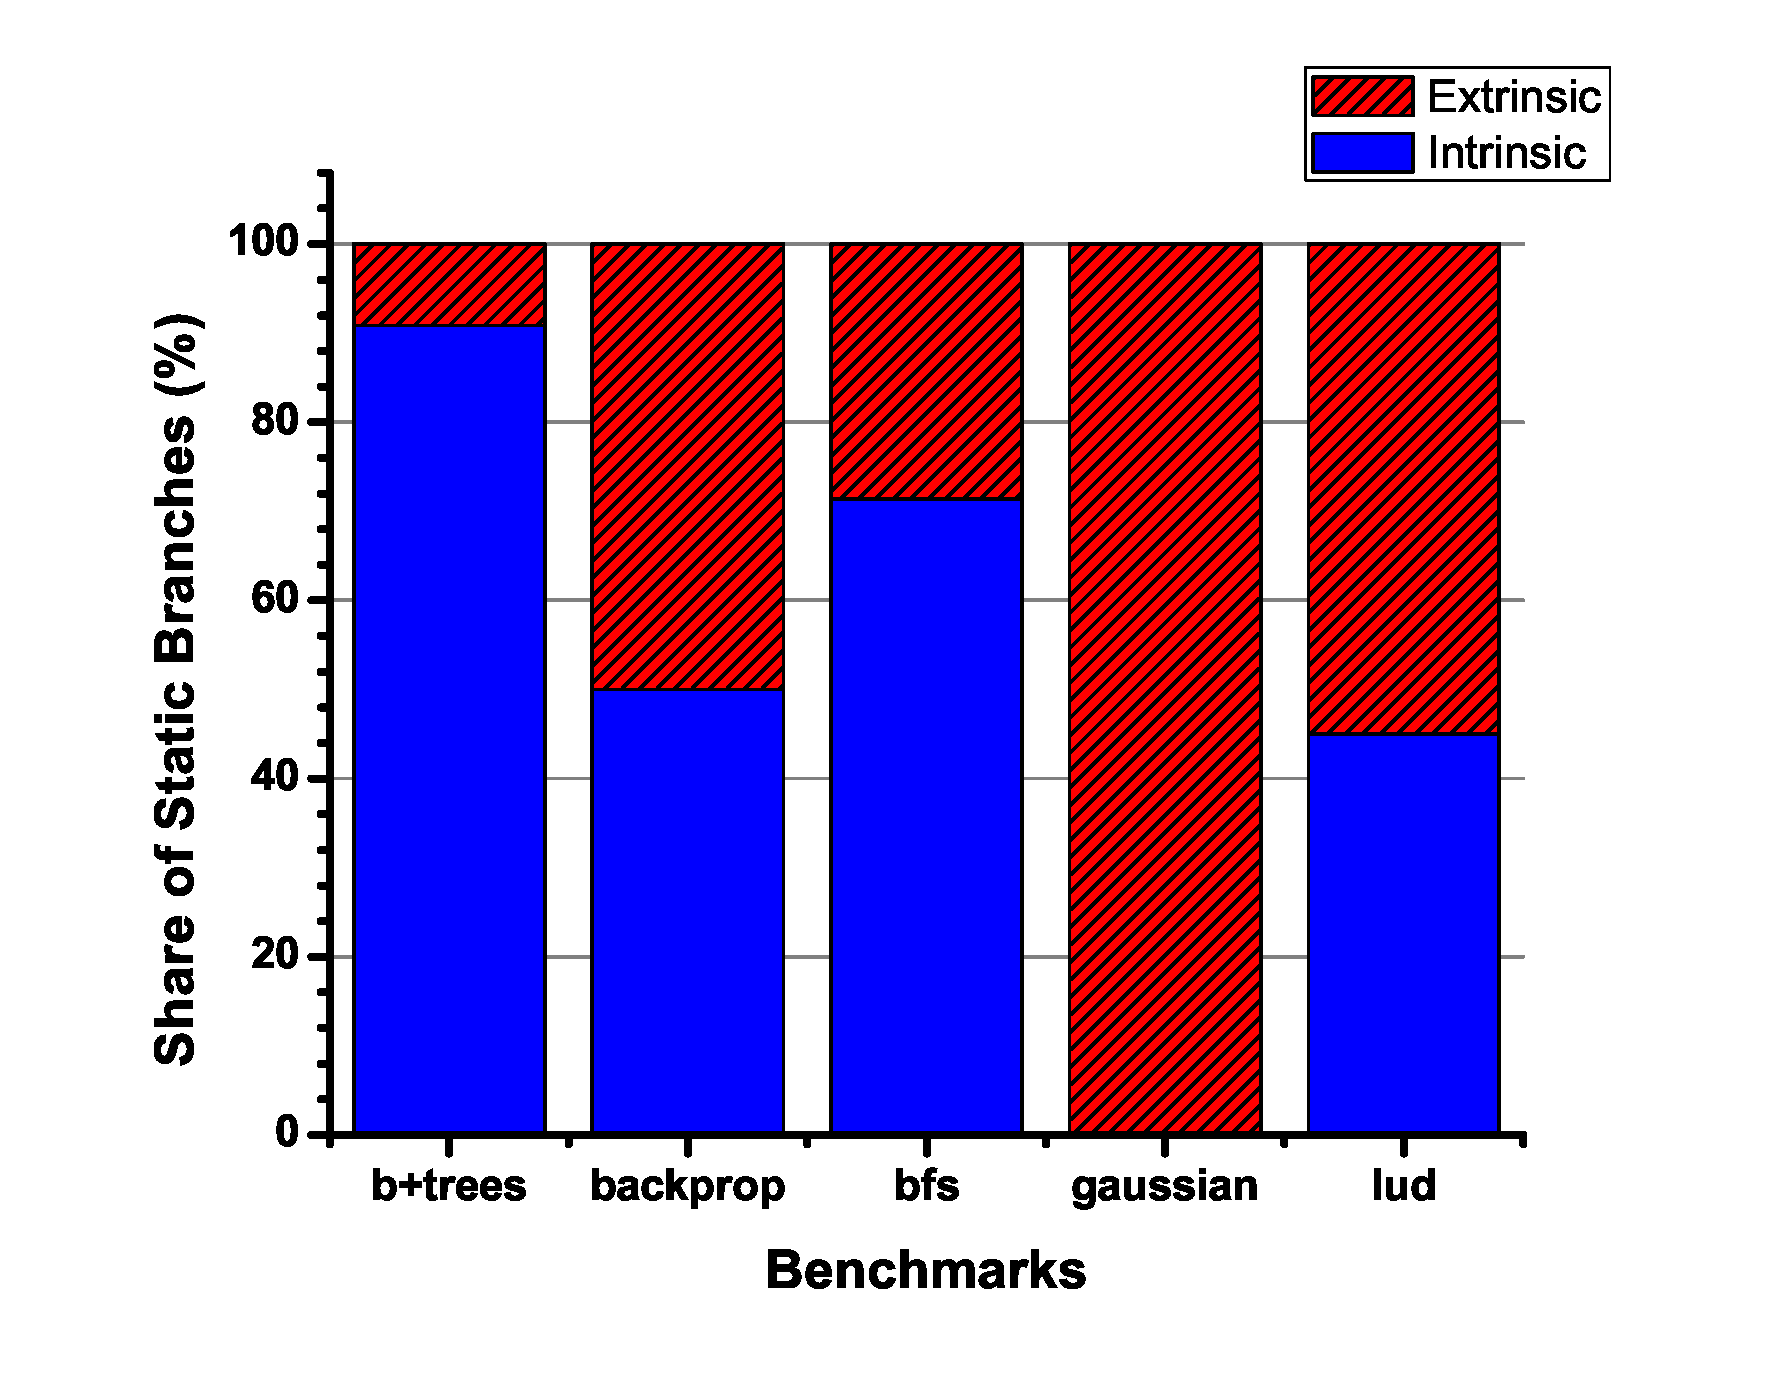
\includegraphics[width=10cm]{static-branches}
		\caption{static count for branch instructions
			\label{fig:static-branches}}
	\end{subfigure}
	\begin{subfigure}{0.45\textwidth}
		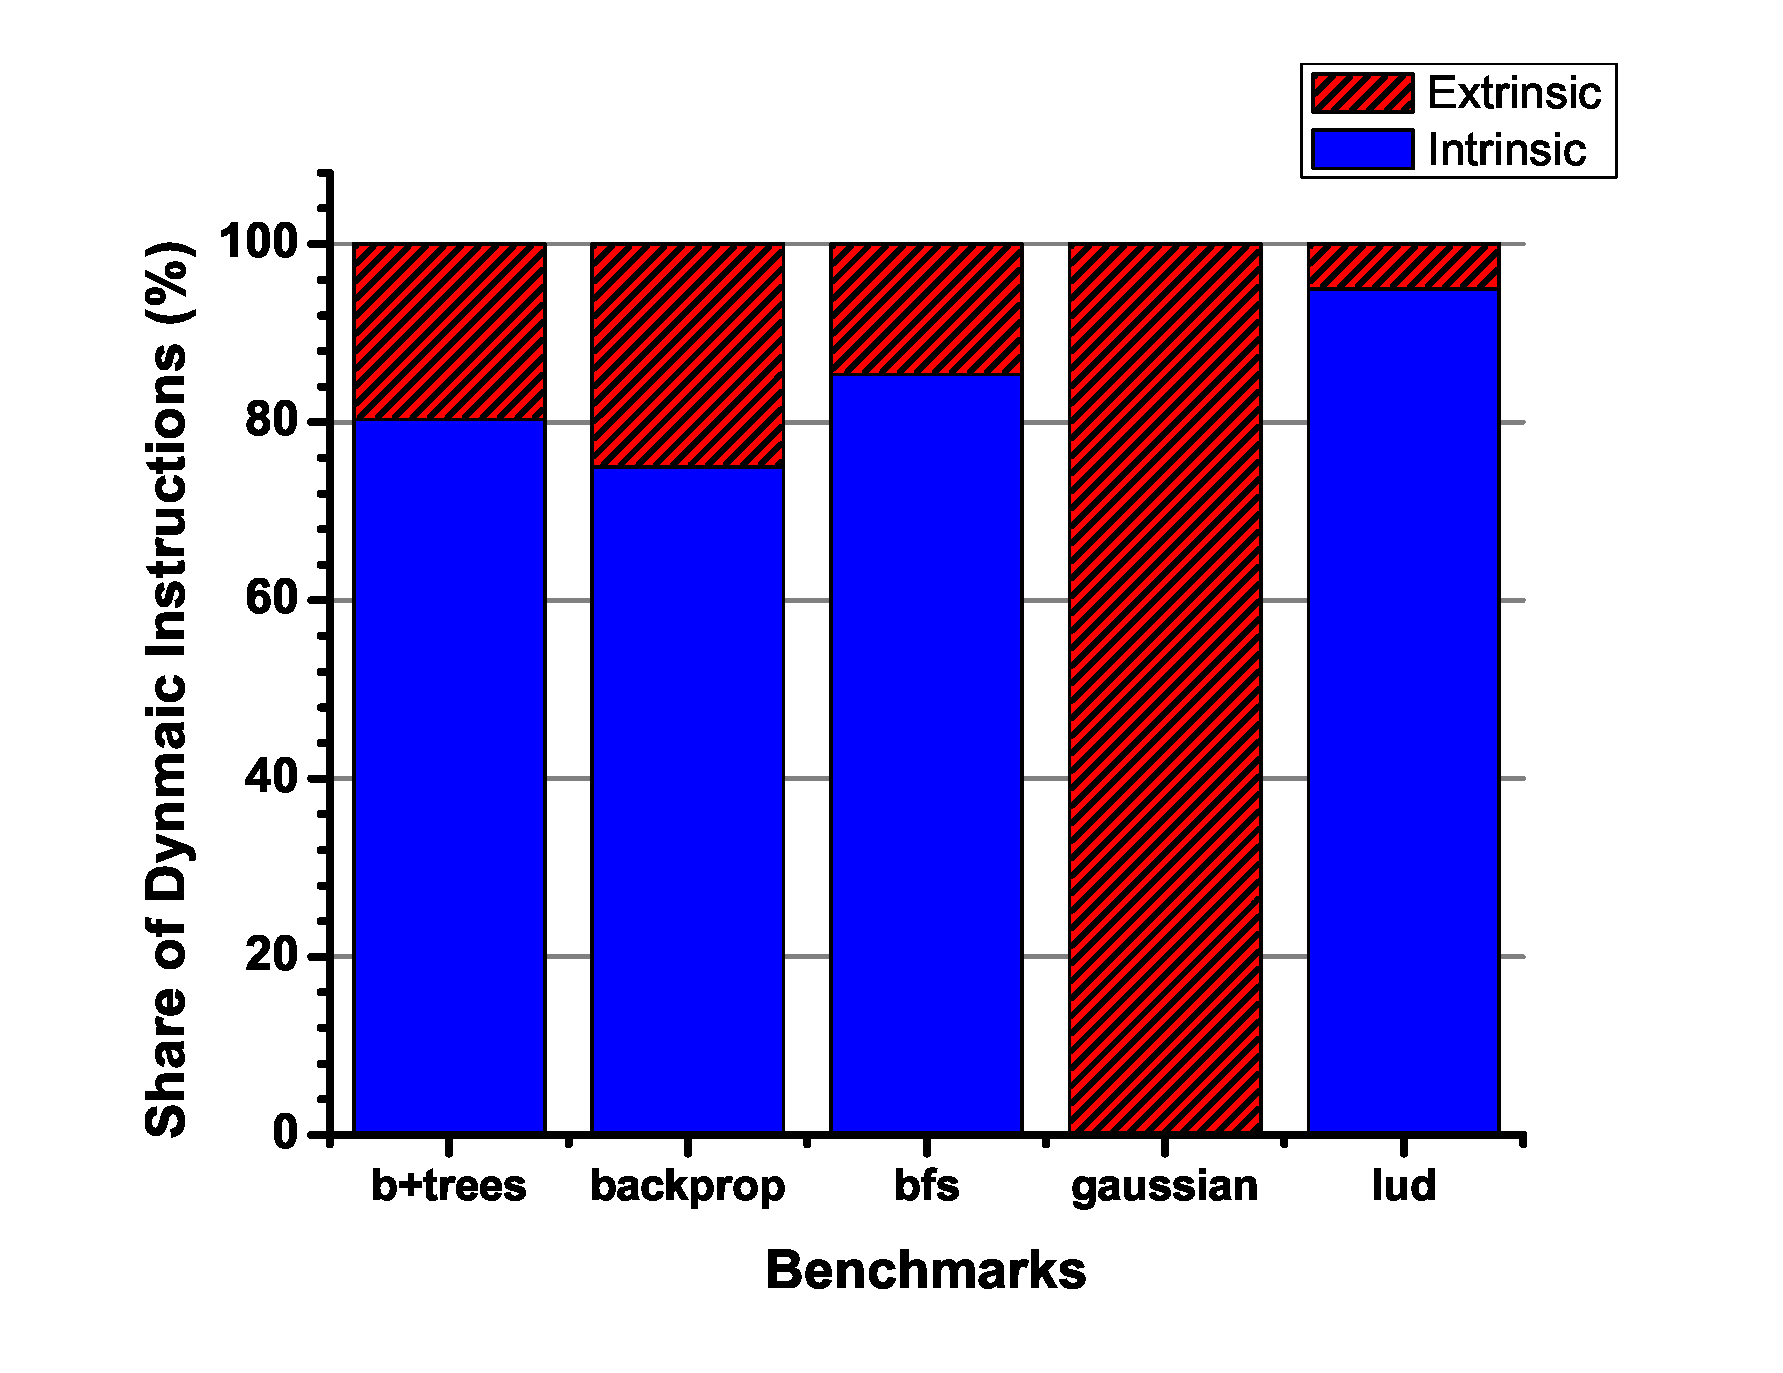
\includegraphics[width=10cm]{dynamic-branches}
		\caption{dynamic count for branch instructions
			\label{fig:dynamic-branches}}
	\end{subfigure}
	\caption{Distribution of the number of branches encountered in different benchmarks
		\label{fig:static-dynamic-distribution-plot}}
\end{figure*}
	Figure \ref{fig:static-dynamic-distribution-plot} shows the distribution of intrinsic and extrinsic branch instructions in terms of their static and dynmaic counts. Static counts are measured by analyzing the compiled ptx code, whereas, the dynamic count is obtained from the branch target buffer shown in Figure \ref{fig:btb-example}.

\subsection{Performance impact}
\begin{figure}
	\centering
	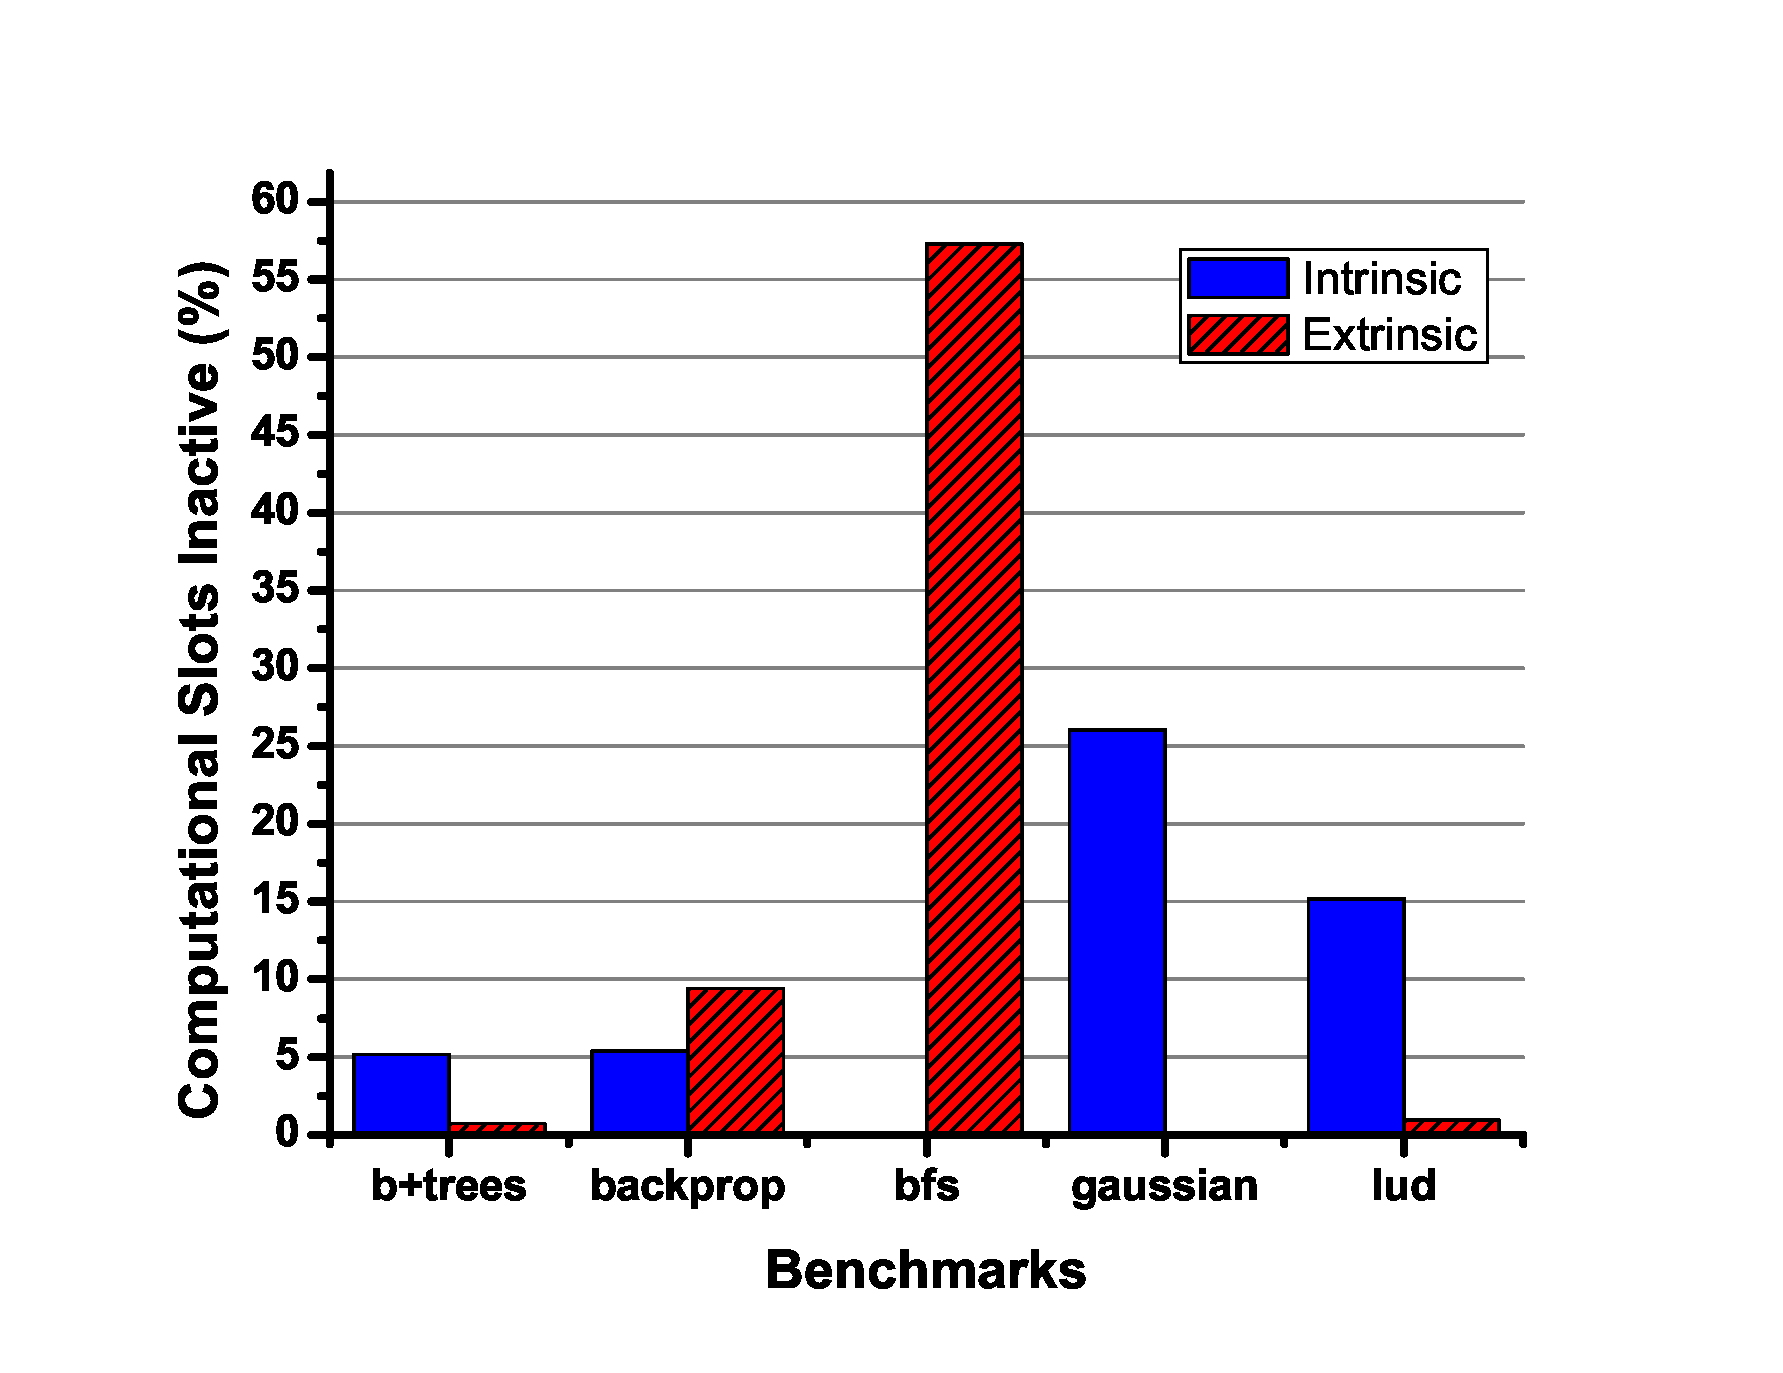
\includegraphics[width=10cm]{computational-slots-wasted}
	\caption{Percentage of computational slots wasted by the two categories of branch instructions
		\label{fig:computational-slots-wasted}}
\end{figure}
As described in Sections \ref{sec:problem-description} and \ref{sec:our-approach}, for each ptx instruction, we measure the total number of slots that were 1. Active, 2. Inactive due to an intrinsic branch and 3. Inactive due to an extrinsic branch. Finally, for any benchmark, we evaluate the aggregate of these metrics over the entire period of time when the benchmark was running. In Figure \ref{fig:computational-slots-wasted}, we report the fraction of total available slots that were wasted due to intrinsic and extrinsic branches respectively.

\subsection{Branch characteristics}
\begin{figure}
	\centering
	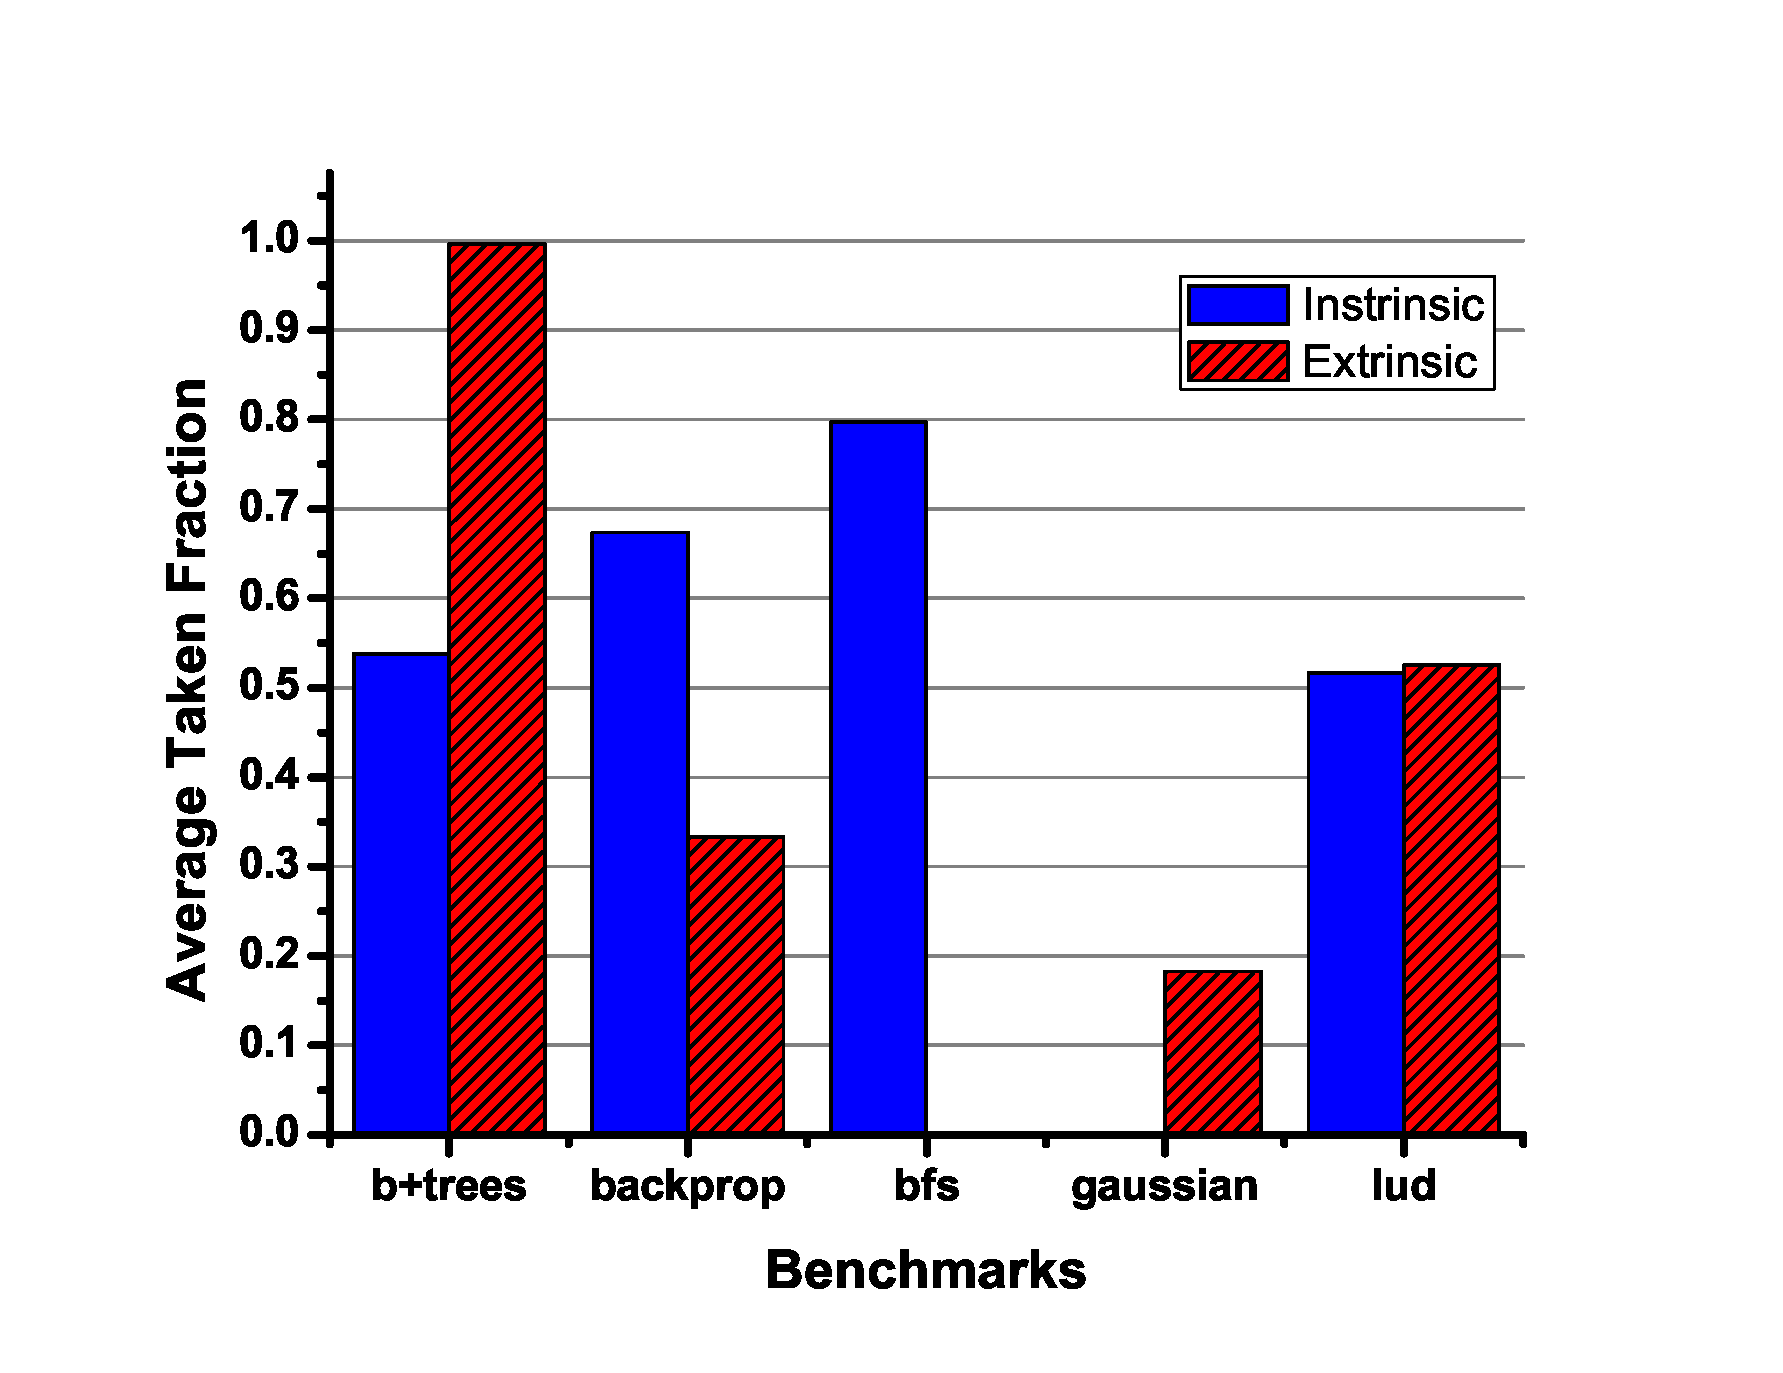
\includegraphics[width=10cm]{taken-fraction}
	\caption{Characterizing extrinsic and intrinsic branches based on the fraction of times they are taken when encountered
		\label{fig:taken-fraction}}
\end{figure}
In Figure \ref{fig:taken-fraction}, we report the weighted average of taken fractions (normalized by the instances for each branch, as reported in Figure \ref{fig:btb-example}) for each class of branches.

